Det är under dessa år som Spotify först når en affärsplattform. Det görs stora återinvesteringar och företaget växer så det knakar. 

\subsection{Idé}
Grundtanken med Spotify förblir att strömma musik till människor. 

\subsection{Produkt}
Det är under 2010 som Spotify börjar få ordning på sin produkt och den blir mer lik det som finns idag. Man släpper det tidigare behovet av en inbjudan i och med att man lanserar Spotify Open. Det blir alltså fritt fram för alla att registrera sig och börja lyssna. Mellan låtarna får man stå ut med reklam men det är en balanserad mängd som många kan stå ut med. 

För dem som inte står ut med reklam finns fortfarande Spotify Premium som innebär att man inte behöver ta del av någon reklam och att 
ljudkvaliteten förbättras från 160 kbps till 320 kbps. 

Det släpps nu även ytterligare en version, Spotify Unlimited, som utöver det som Premium har att erbjuda även möjliggör lyssning av Spotify i mobiltelefonen.

%Här vill jag ha en tabel

Att dela med sig av sin musik är något som efterfrågas och Spotify får upp ögonen för. Man inför en rad sociala möjligheter för att kunna dela låtar och spellistor med sina vänner direkt i Spotify. 

Under 2011 tar Spotify ett utmanande kliv mot bland annat iTunes när man inför möjligheten att köpa enskilda låtar och album. Det går nu även att lägga in annan musik som man har på sin hårddisk så att Spotify blir ett komplett ljudbibliotek för din dator. En funktion för att synkronisera detta med sin iPod gör Spotify till stark utmanare av Apples iTunes.

Senare under samma år införs en App Store i Spotify som möjliggör för tredjepartsutvecklare att föra in program i musikspelaren med diverse features. Det handlar väldigt ofta om att rekomendera musik. Alla stora musikredaktioner, till exempel Rolling Stone Magasize eller svensk P3, har sin app där de rekomenderar, resencerar och delar sina tankar. Andra populära funktioner är bland annat TuneWiki som levererar texten till musik du lyssnar på.

\subsection{Marknad}
Väldigt svårt att få en oberoende analys av.

\subsection{Organisation}
Stor

\subsection{Erfarenhet}
Spotify är för många en mycket attraktiv arbetsgivare varför de lockar till sig många intresserade arbetstagare. Det borde därför inte vara svårt att anställa folk med önskad kompetens. 

\subsection{Engagemang}
Tillräckligt

\subsection{Relation till kunder}
Hmm

\subsection{Relation till andra företag}
Det lades mycket fokus på att knyta kontakter med företag på andra marknader. Det skrevs avtal med bland annat Facebook och Coca-Cola. Detta gjorde Spotify konkurrenskraftiga gentemot andra musiktjänster och gav dem även möjlighet att växa sig större snabbare. Genom att synas tillsammans med stora etablerade företag i diverse reklamkampanjer och liknande kunde även Spotifys eget varumärke förstärkas. 

Samarbetet med Facebook kan anses vara av extra stor vikt. Möjligheterna att dela med sig av sin musik och se vad andra lyssnar på blev helt plötsligt enorma. I samband med att Spotify presenterades på Facebooks F8 konferens sågs till exempel en ökning av månatliga aktiva användare på en miljon. 

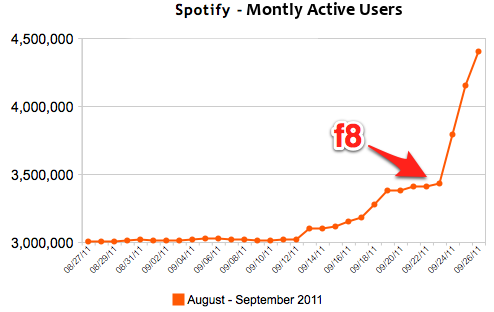
\includegraphics[width=\linewidth]{images/MAU2011.png}
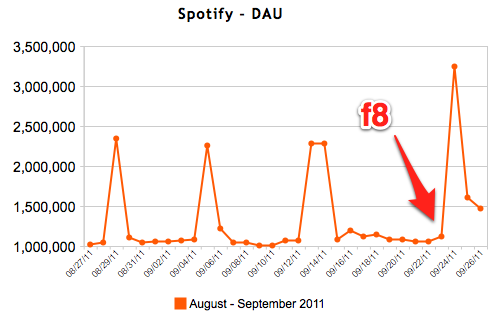
\includegraphics[width=\linewidth]{images/DAU2011.png}

Nedan följer en lista med företag Spotify på något vis samarbetat med:

\begin{itemize}
  \item \emph{Telia}, Sverige - 2009. \\
Få sex månader gratis premium. Förde in Spotify i Telias många butiker i Sverige och även på deras hemsida.

\item \emph{SFR}, Frankrike - 2009. \\
Spotify ingår som del i månadskostnaden. Spotify syns på deras hemsida.

\item \emph{Nissan}, Japan - 2009. \\
Nissan Quasquai var Powered By Spotify. Detta visades för alla intresserade kunder på hemsida.

\item \emph{Sonos}, USA	- 2010.\\
Spotifys första hårdvaruintegration. Sonos är en Amerikansk hi-fi-aktör inriktad mot trådlösa musiksystem. Sonos närvarar på över 60 marknader.

\item \emph{Chevrolet}, USA	- 2011.\\
De första 150 000 som började prenumerera på Chevrolet på Facebook fick en Spotify inbjudan. Detta skedde under den tid då inbjudan krävdes för att få tillgång till Spotify.

\item \emph{Onkyo}, Japan - 2011.\\
Japansk hi-fi aktör som var först med att erbjuda Spotify genom deras hemmabioanläggning.

\item \emph{Logitech}, USA - 2011.\\
Spotify infördes i Logitechs Squeezebox, en nätverksmusikenhet. Detta möjliggör för streaming från Spotify och uppspelning av spellistor. Logitech tillverkar datortillbehör och annan musikutrustning.

\item \emph{Facebook}, USA - 2011.\\
Spotify integreras i Facebook och vice-versa. Man kan lyssna på musik direkt i Facebook, dela spellistor och se vad kompisar lyssnar på.

\item \emph{Shazam}, Storbrittanien - 2011.\\
En tjänst lik sound hound som "lyssnar" på en låt och säger vad den heter. Detta kopplades ihop med Spotify så att låten direkt kan spelas via deras bibliotek.

\item \emph{SEAT}, Spanien - 2011. \\
Få en Samsung mobil med Spotify installerat gratis i sex månader. Reklam syntes på TV, billboards, youtube, tidningar, hemsida.

\item \emph{Coca-Cola}, USA	- 2012.\\
Sammarbete med Coca-Cola can vara mycket lönsamt då de är aktiva i cirka 200 länder vilket för ut Spotify på nya marknader. Samtidigt kan Spotify bistå med musik till Coca-Colas online-marknadsföring på till exempel Facebook.

\item \emph{Virgin Mobile}, Storbrittanien - 2012. \\
Få tre månaders gratis premium. Spotify syns på deras hemsida.

\item \emph{Volkswagen}, Tyskland - 2012.\\
Spotify musik spelas på Volkswagens hemsida och folk kan önska musik som ska spelas. Spotifys logo syns tydligt och binder samman de två företagen.
\end{itemize}
